% Chapter Template

\chapter{FDTD - Two-Dimensional Scenario} % Main chapter title

\label{Chapter3} % Change X to a consecutive number; for referencing this chapter elsewhere, use \ref{ChapterX}

%----------------------------------------------------------------------------------------
%	SECTION 1
%----------------------------------------------------------------------------------------

Now that the one-dimensional scenario is complete, the following is going to be much easier, as for the most part the same logic is going to be used again. For the interest of saving time, redundant information that was covered previously is going to be omitted.

\section{2D Discretization}

In the previous chapter the different transverse modes available for electromagnetic waves were mentioned briefly without going too much in depth as they were not so relevant in that scenario. In a one-dimensional case, it does not matter much which axis is picked for which field, so long as they are perpendicular to each other. In the two-dimensional scenario however, the mode that is choosen is going to dictate the curls that will be used. 

\subsection{2D Transverse Modes}

For the two-dimensional scenarios, choosing a transverse mode means that the chosen field will have no vectors in the direction of propagation, meaning the $z$ axis in this case. That means that any vector moving along that axis will have a value of zero for that field. However, the other field can only have values alongside that direction, meaning that it will be zero for the $x$ and $y$ axis instead. More specifically, each mode features the following field vectors:

\begin{itemize}
	\item \textbf{TE mode} - \space $E_x,\; E_y,\; H_z$
	\item \textbf{TM mode} - \space $E_z,\; H_x,\; H_y$
\end{itemize}

While each mode will have different vectors, the process is roughly the same. For this scenario TE mode will be used, meaning that $E_z, H_x, H_y = 0$.

\subsection{2D TE Electromagnetic Curls}

Similar to the one-dimensional scenario, each vector will have a curl around it, such as the $H_z$ vector in figure \ref{fig:fdtd2dHz}:

\begin{figure}[h!]
	\centering
	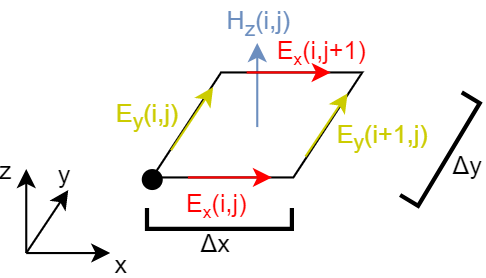
\includegraphics[scale=0.6]{Figures/fdtd2dHz}
	\decoRule
	\caption[2D TE Mode - $H_z$ vector curl]{The curl around the magnetic field vector $H_z$.}
	\label{fig:fdtd2dHz}
\end{figure}

Using a similar indexing scheme as done previously:

\begin{equation}
	\label{eqn:indexing2DElectric}
	E_{i,j} = E(i \cdot \Delta x , j \cdot \Delta y)
\end{equation}

\begin{multline}
	\label{eqn:2dHzCurl1}
	\oint \vec{E} \cdot d\vec{s} = - \frac{d}{dt} \iint \mu \cdot \vec{H} \cdot d\vec{A} \\
	\Rightarrow E_x(i,j) \cdot \Delta x - E_x(i,j+1) \cdot \Delta x + E_y(i+1,j) \cdot \Delta y - E_y(i,j) \cdot \Delta y \\ = -\frac{d}{dt}(\mu \cdot H_z(i,j) \cdot \Delta x \cdot \Delta y)
\end{multline}

which leads to

\begin{equation}
	\label{eqn:2dHzCurl2}
	\frac{d}{dt} H_z(i,j) = -\frac{1}{\mu} \cdot (\frac{E_x(i,j) - E_x(i,j+1)}{\Delta y} + \frac{E_y(i+1,j)- E_y(i,j)}{\Delta x})
\end{equation}

If there is a uniform mesh size, meaning that $\Delta x = \Delta y =  \Delta z = \Delta s$, one can simplify equation \ref{eqn:2dHzCurl2} to:

\begin{equation}
	\label{eqn:2dHzCurl3}
	\frac{d}{dt} H_z(i,j) = -\frac{1}{\mu \cdot \Delta s} \cdot ((E_x(i,j) - E_x(i,j+1) + E_y(i+1,j)- E_y(i,j))
\end{equation}

For the left hand side, it is known that:

\begin{equation}
	\label{eqn:2dHzCurl4}
	\frac{d}{dt} H_z(i,j) = \frac{H_z^{new}(i,j) - H_z^{prev}(i,j)}{\Delta t}
\end{equation}

Combining equations \ref{eqn:2dHzCurl3} and \ref{eqn:2dHzCurl4} results in the update equation for the magnetic field vector $H_z$:

\begin{multline}
	\label{eqn:2dHzCurlFinal}
	H_z^{new}(i,j) =  H_z^{prev}(i,j) -\frac{\Delta t}{\mu \cdot \Delta s} \cdot \\ (E_x(i,j) - E_x(i,j+1) + E_y(i+1,j)- E_y(i,j))
\end{multline}

For the electric vectors $E_x$ and $E_y$, the equations and curls are going to be roughly the same as the ones for the one-dimensional scenario. The curl for $E_x$ can be seen in Figure \ref{fig:fdtd2dEx}:

\begin{figure}[h!]
	\centering
	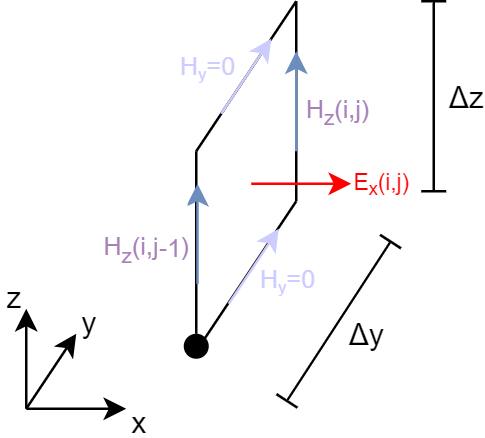
\includegraphics[scale=0.6]{Figures/fdtd2dEx}
	\decoRule
	\caption[2D TE Mode - $E_x$ vector curl]{The curl around the electric field vector $E_x$.}
	\label{fig:fdtd2dEx}
\end{figure}

resulting in the following update equation:

\begin{equation}
	\label{eqn:2dExCurlFinal}
	E_x^{new}(i,j) =  E_x^{prev}(i,j) + \frac{\Delta t}{\epsilon \cdot \Delta s} \cdot (H_z(i,j) - H_z(i,j-1))
\end{equation}

In a similar fashion, the curls for $E_y$ will be as follows (Figure \ref{fig:fdtd2dEy}),

\begin{figure}[h!]
	\centering
	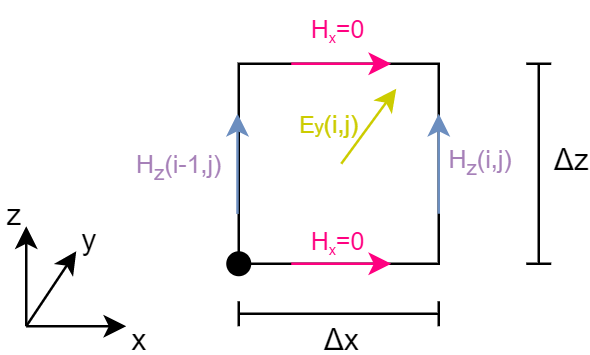
\includegraphics[scale=0.6]{Figures/fdtd2dEy}
	\decoRule
	\caption[2D TE Mode - $E_y$ vector curl]{The curl around the electric field vector $E_y$.}
	\label{fig:fdtd2dEy}
\end{figure}

with a fairly similar equation (note the signs):

\begin{equation}
	\label{eqn:2dEyCurlFinal}
	E_y^{new}(i,j) =  E_y^{prev}(i,j) - \frac{\Delta t}{\epsilon \cdot \Delta s} \cdot (H_z(i,j) - H_z(i-1,j))
\end{equation}

The code implementation can now begin.

\section{C++ Implementation}

Starting off with the imports, the ones that were already discussed will not be explained again. There are however new headers that will be needed:

\begin{minted}[breaklines,frame=single,fontsize=\footnotesize]{c++}
#include <io.h>
#include <fstream>
\end{minted}

For the two dimensional scenario, a new method of visualizing the data will be used. The end result will be an animation that shows how the waves propagate in real time. It will be explained more in depth once data visualization is described, but for now all that is needed to be known is that the output of the two-dimensional implementation is going to be CSV files that contain the data. The header files above will help with that:

\begin{itemize}
	\item \textbf{fstream}\textsuperscript{\cite{fstream}} - Input output stream operations for files. Allows users to create and modify them.
	\item \textbf{io.h}\textsuperscript{\cite{io.h}} - Header file used by \textbf{fstream} among other standard library files.
\end{itemize}

Two new C++ functions to write the electromagnetic data into files need to be introduced:

\begin{minted}[breaklines,frame=single,fontsize=\footnotesize]{c++}
void writeEDataToCsvFile(string filename, const vector<vector<double>> &Ex, const vector<vector<double>> &Ey){
	
	//	x,y,z,Ex,Ey
	//	i,j,0,Ex[x,y],Ey[x,y]
	
	ofstream csvFile(filename);
	csvFile << "x,y,z,Ex,Ey\n";
	
	for (unsigned x = 0; x < Ex[0].size(); x++) {
		for (unsigned y = 0; y < Ex[x].size(); y++) {
			csvFile << to_string(x) + "," + to_string(y) + ",0," + to_string(Ex[x][y]) + "," + to_string(Ey[x][y]) + "\n";
		}
	}
	
	csvFile.close();
}

void writeHDataToCsvFile(string filename, const vector<vector<double>> &Hz){
	
	//	x,y,z,Hz
	//	i,j,0,Hz[x,y]
	
	ofstream csvFile(filename);
	csvFile << "x,y,z,Hz\n";
	
	for (unsigned x = 0; x < Hz[0].size(); x++) {
		for (unsigned y = 0; y < Hz[x].size(); y++) {
			csvFile << to_string(x) + "," + to_string(y) + ",0," + to_string(Hz[x][y]) + "\n";
		}
	}
	
	csvFile.close();
}
\end{minted}

These functions will be called every loop to print a file that contains the respective field's data for that time step. The filename format should be \textit{"X.csv.n"}, where \textit{X} is the field the data is for (E for electric, H for magnetic), while \textit{n} is the time step number. These files are going to get added in the the directory: \mint{c++}{const string filePath = "./Out/";}

Some changes need to be made to the code to adapt it to a two-dimensional environment. For starters, the vectors need to be initialized as two-dimensional. The electric field will also require an extra vector now for a total of two, one for the $x$ axis and one for the $y$ axis. In total, the following vectors need to be declared:

\begin{minted}[breaklines,frame=single,fontsize=\footnotesize]{c++}
vector<vector<double>> Ex(N, vector<double> (N, 0));
vector<vector<double>> Ey(N, vector<double> (N, 0));
vector<vector<double>> Hz(N, vector<double> (N, 0));
\end{minted}

Normally one would also need to add new variables for the deltas:
\begin{minted}[breaklines,frame=single,fontsize=\footnotesize]{c++}
double deltaX = L / N;
double deltaY = L / N;
double deltaZ = L / N;
\end{minted}

Since a uniform mesh is being used, meaning all the spatial steps have the same dimensions, only one of these deltas needs to be used (e.g. \textit{deltaZ}). In the Appendix (\ref{AppendixA}) implementations for unequal mesh step sizes will be discussed further. For now, since only one delta will be used, $\Delta t$ will need to be changed to:

\begin{minted}[breaklines,frame=single,fontsize=\footnotesize]{c++}
double deltaT = (deltaZ * sqrt(permitivity*permeability)  * (1/sqrt(2)));
\end{minted}

Another difference is that the Gaussian pulse excitation is going to be applied in the center of the magnetic field this time. Due to the impedance of vacuum, it is prudent to promptly reduce the magnitude of this excitation, as otherwise the electric values would be far too large.

\begin{minted}[breaklines,frame=single,fontsize=\footnotesize]{c++}
// reducing the magnitude since in free space
Hz[99][99] = exp(-(beta * pow((t - gamma), 2))) * 10e-4;
\end{minted}

Starting from the center will result in a nice symmetric propagation towards the edges. In symmetrical scenarios one can save computation time by splitting the domain into equal parts. It is even more helpful with circular symmetry as the domain can effectively be split into as many parts as needed, and by calculating the wave propagation for only one part, those values can be then replicated for the other parts. This will also be discussed in the Appendix.

By translating the update equations into code, the main loop becomes:

\begin{minted}[breaklines,frame=single,fontsize=\footnotesize]{c++}
for (int i = 0; i < N-1; i++) {
	for (int j = 1; j < N-1; j++) {
		Ex[i][j] = Ex[i][j] + (deltaT / permitivity / deltaZ) * (Hz[i][j] - Hz[i][j-1]);
	}
}

for (int i = 1; i < N-1; i++) {
	for (int j = 0; j < N-1; j++) {
		Ey[i][j] = Ey[i][j] - ((deltaT / permitivity / deltaZ) * (Hz[i][j] - Hz[i-1][j]));
	}
}
writeEDataToCsvFile((filePath + "E/E.csv." + to_string(i)), Ex, Ey);

// loop for values
for (int i = 0; i < N-2; i++) {
	for (int j = 0; j < N-2; j++) {
		Hz[i][j] = Hz[i][j] - ((deltaT / permeability / deltaZ) * (Ex[i][j] - Ex[i][j+1] + Ey[i+1][j] - Ey[i][j]));
	}
}
writeHDataToCsvFile((filePath + "H/H.csv." + to_string(i)), Hz);
\end{minted}

After each vector field is done, one can call the respective method to write the data into csv files. For organizational purposes, this data will be dumped into separate folders for each field. After waiting for code execution to finish, there will now be two folders with data that is ready to be used for visualization.

\section{Data Visualization}

In order to visualize two-dimensional data in a meaningful manner, it would help to use an open source program called Paraview\textsuperscript{\cite{paraview}}. It allows to build animated visualizations with the data that was generated. It is also the reason for the chosen naming scheme for the output files. By using the format \textit{X.csv.n} they can all be imported as one object. This can be easily done by simply opening Paraview, selecting all of the data in one of the output folders, and just dragging and dropping it into the "Pipeline Browser" panel, pictured below (Figure \ref{fig:paraviewFDTD2D1}).

\begin{figure}[h!]
	\centering
	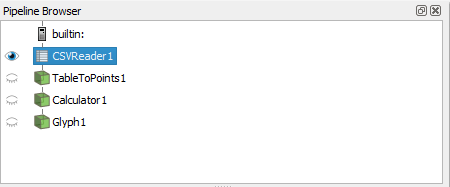
\includegraphics[scale=0.6]{Figures/paraviewFDTD2D1}
	\decoRule
	\caption[2D TE Mode - $E_x$ vector curl]{The curl around the electric field vector $E_x$.}
	\label{fig:paraviewFDTD2D1}
\end{figure}

Having just the data by itself will not do much however. That is why one needs to apply filters to the data. The ones that will be used in this case are the following:

\begin{itemize}
	\item \textbf{Table to Points} - Simply displays the CSV data as points.
	\item \textbf{Calculator} - Allows to manipulate the data and dictate which value goes where.
	\item \textbf{Glyph} - Transforms the data into lines which are better in visualizing vector fields
\end{itemize}

The order is important, as is the fact that each of these filters must be configured properly. For \textbf{Table to Points}, the vector components for the data needs to be defined. In the output files, one will notice that not only $x$ and $y$ have been specified, but also $z$, which contains only zeros. That needed to be done that since Paraview will not accept less than three columns here. It is also helpful to tick \textbf{Axes Grid} under the \textbf{Annotations} category. In the \textbf{Calculator}, one needs to add the following formula \mint{java}{iHat*Ex+jHat*Ey} which will build the vector data from the components. Lastly, for the \textbf{Glyph}, the \textbf{Result} array gotten from the \textbf{Calculator} needs to be used as both \textbf{Orientation} and \textbf{Scaling}. Depending on whether the data is visible or not,the scaling slider can be changed as desired. If done correctly, one will get a result similar to Figure \ref{fig:FDTD2DE}.

\begin{figure}[h!]
	\centering
    \begin{subfigure}{.49\textwidth}
    	\centering
    	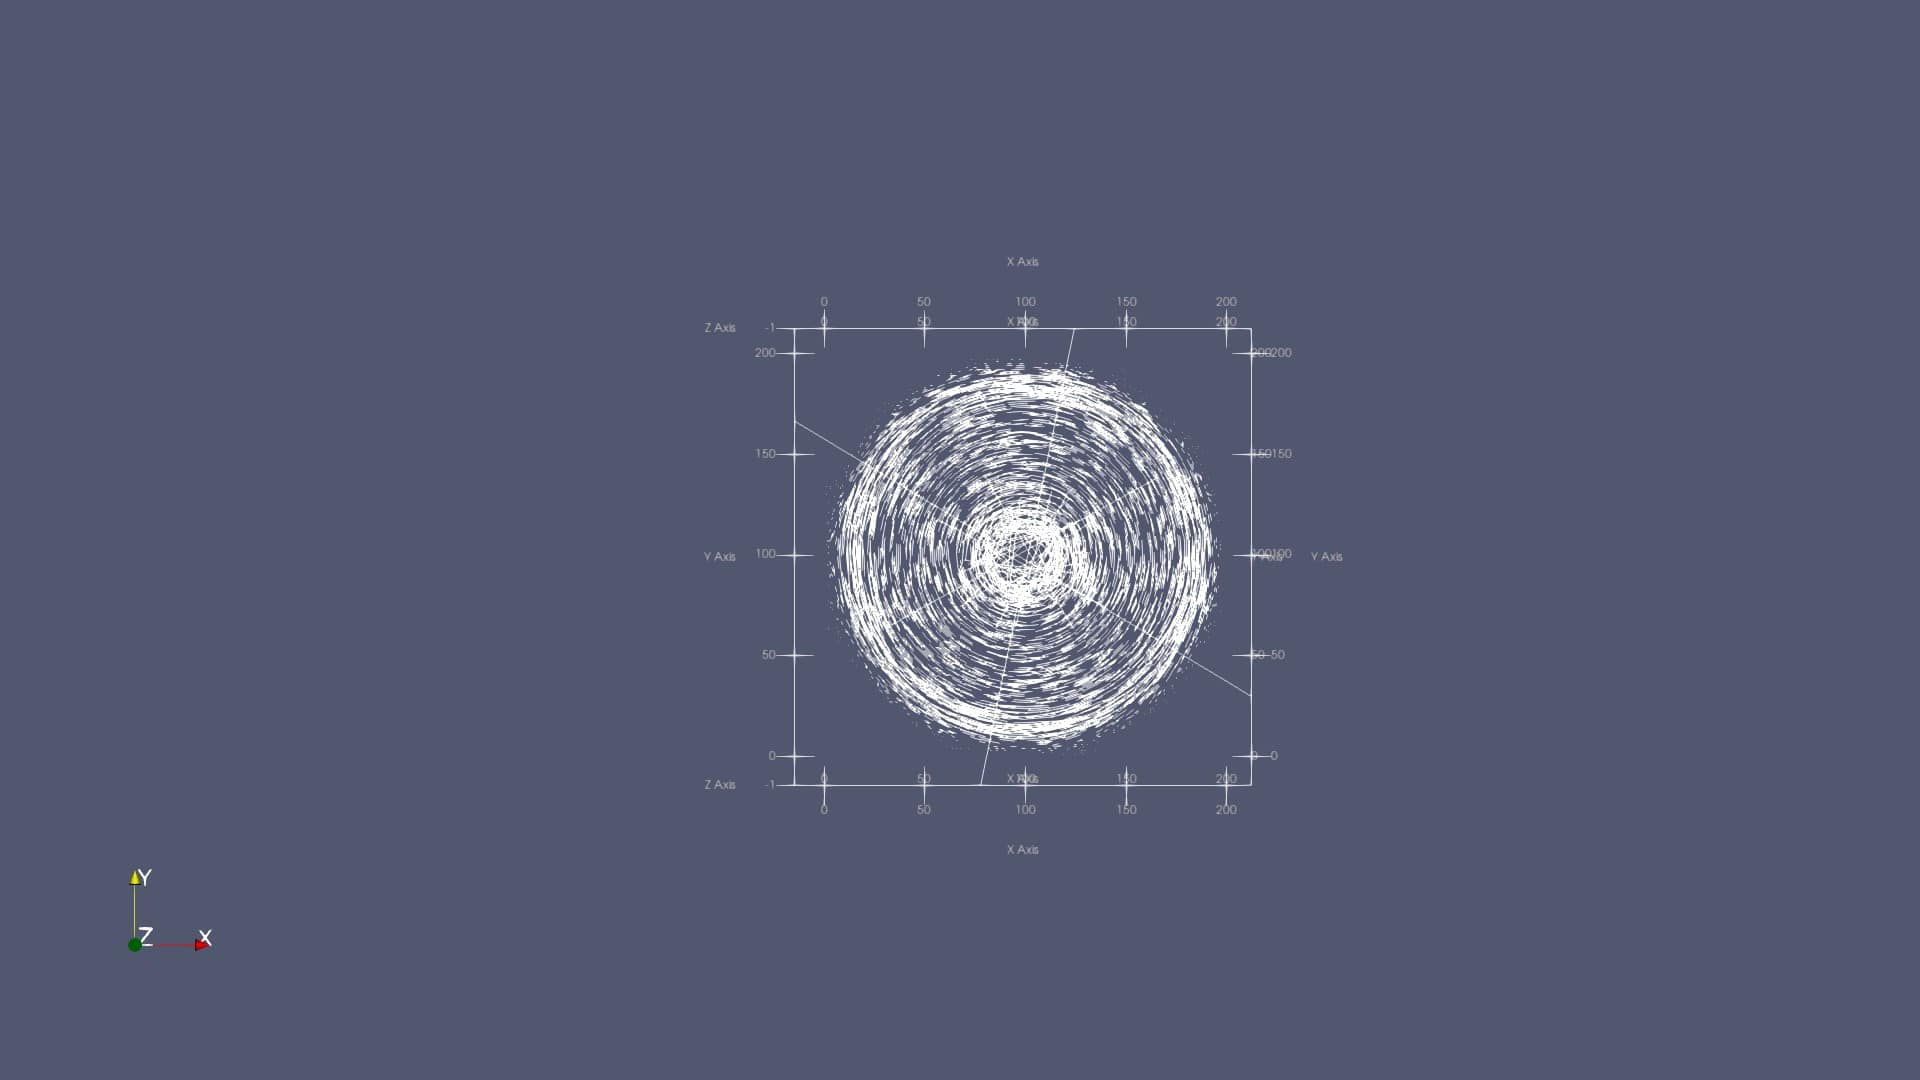
\includegraphics[width=.95\linewidth]{Figures/FDTD2DE1}
    	\caption{t = 200}
    \end{subfigure}
    \begin{subfigure}{.49\textwidth}
    	\centering
    	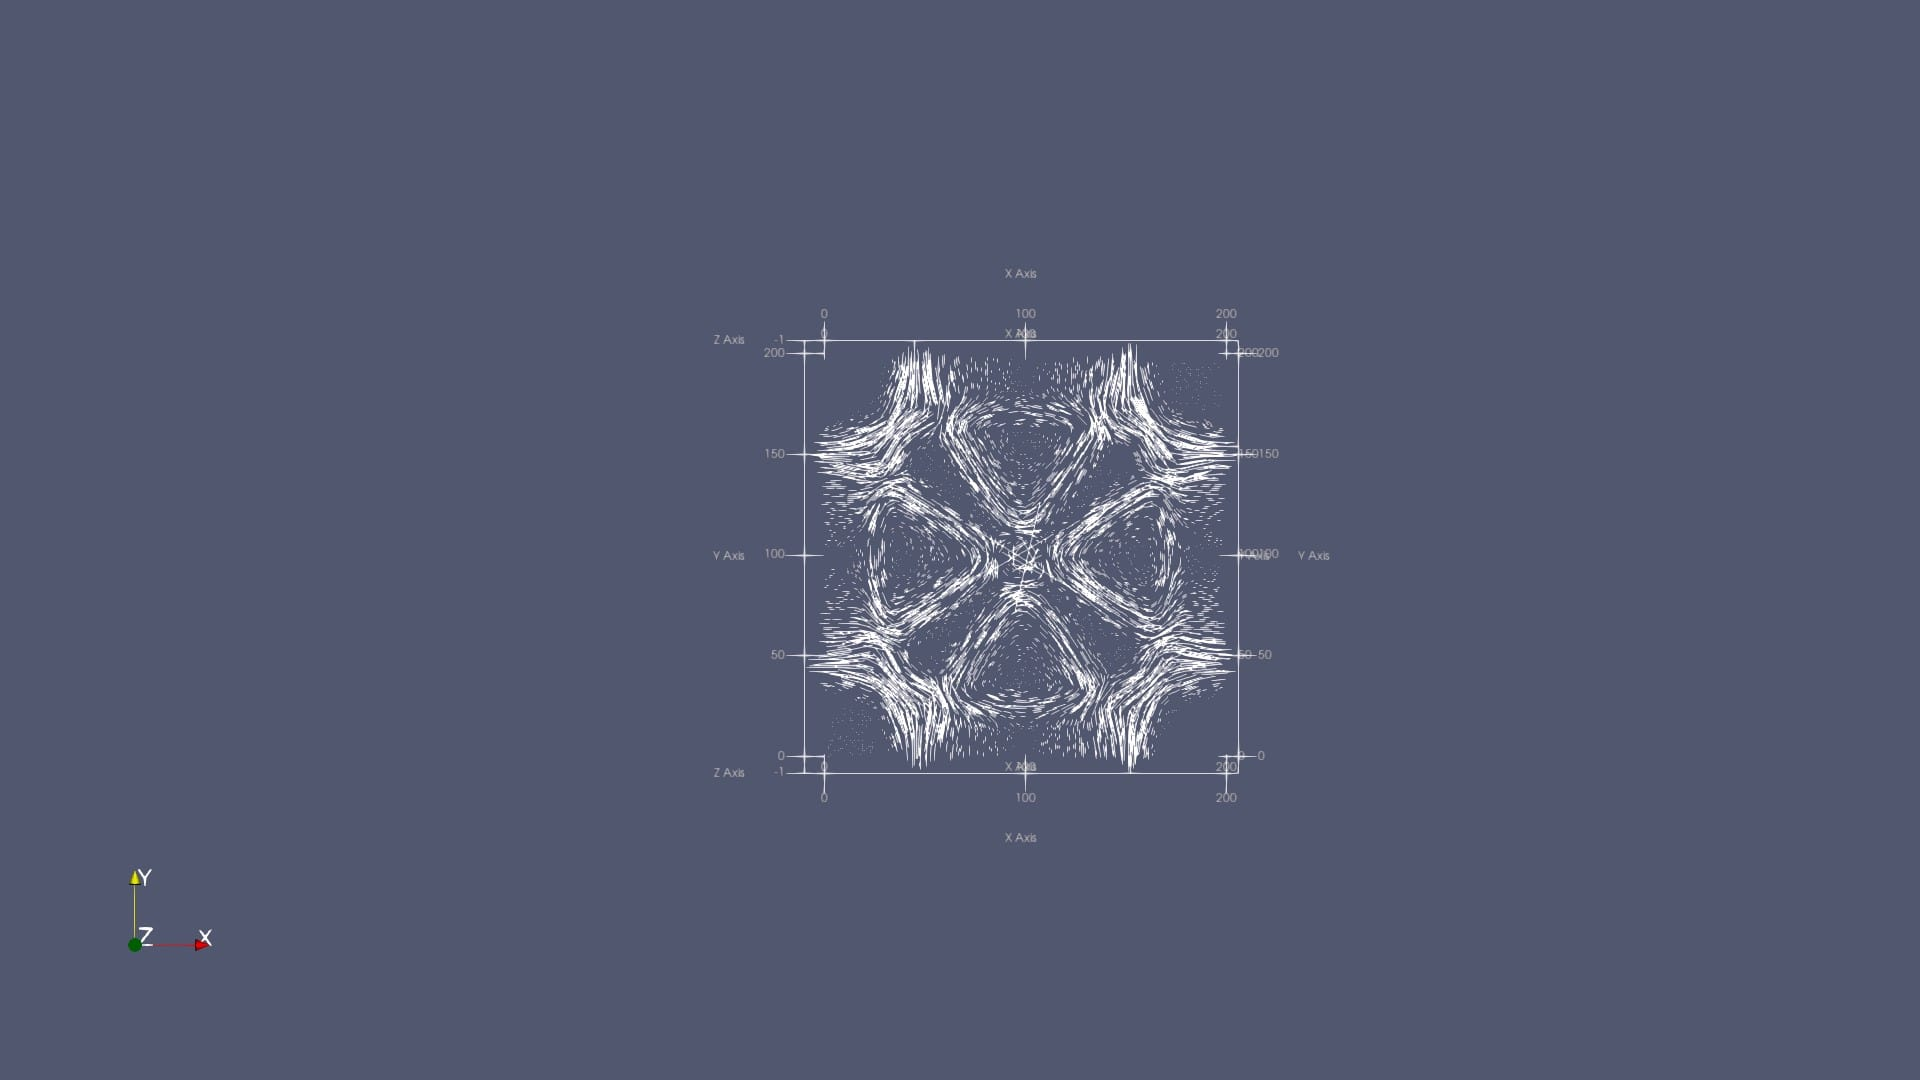
\includegraphics[width=.95\linewidth]{Figures/FDTD2DE2}
    	\caption{t = 400}
    \end{subfigure}
    \begin{subfigure}{.49\textwidth}
    	\centering
    	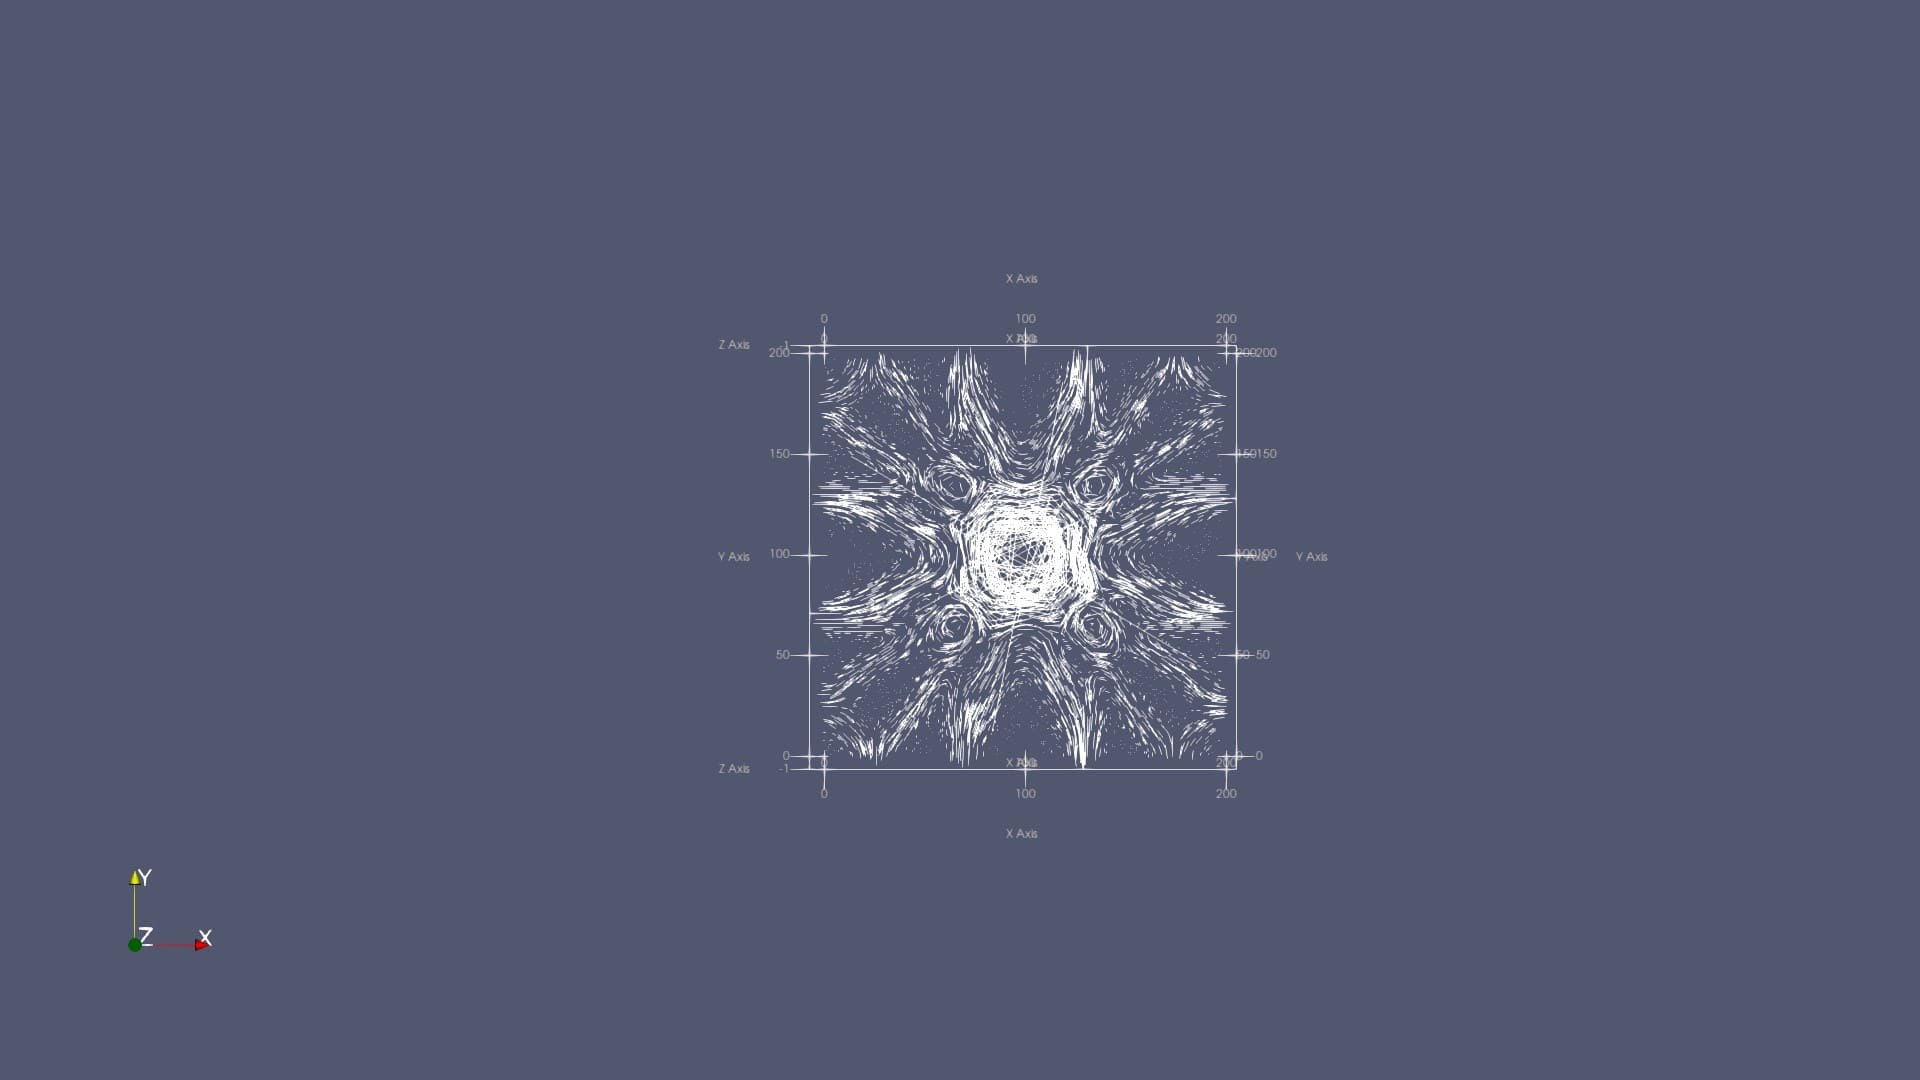
\includegraphics[width=.95\linewidth]{Figures/FDTD2DE3}
    	\caption{t = 600}
    \end{subfigure}
    \begin{subfigure}{.49\textwidth}
    	\centering
    	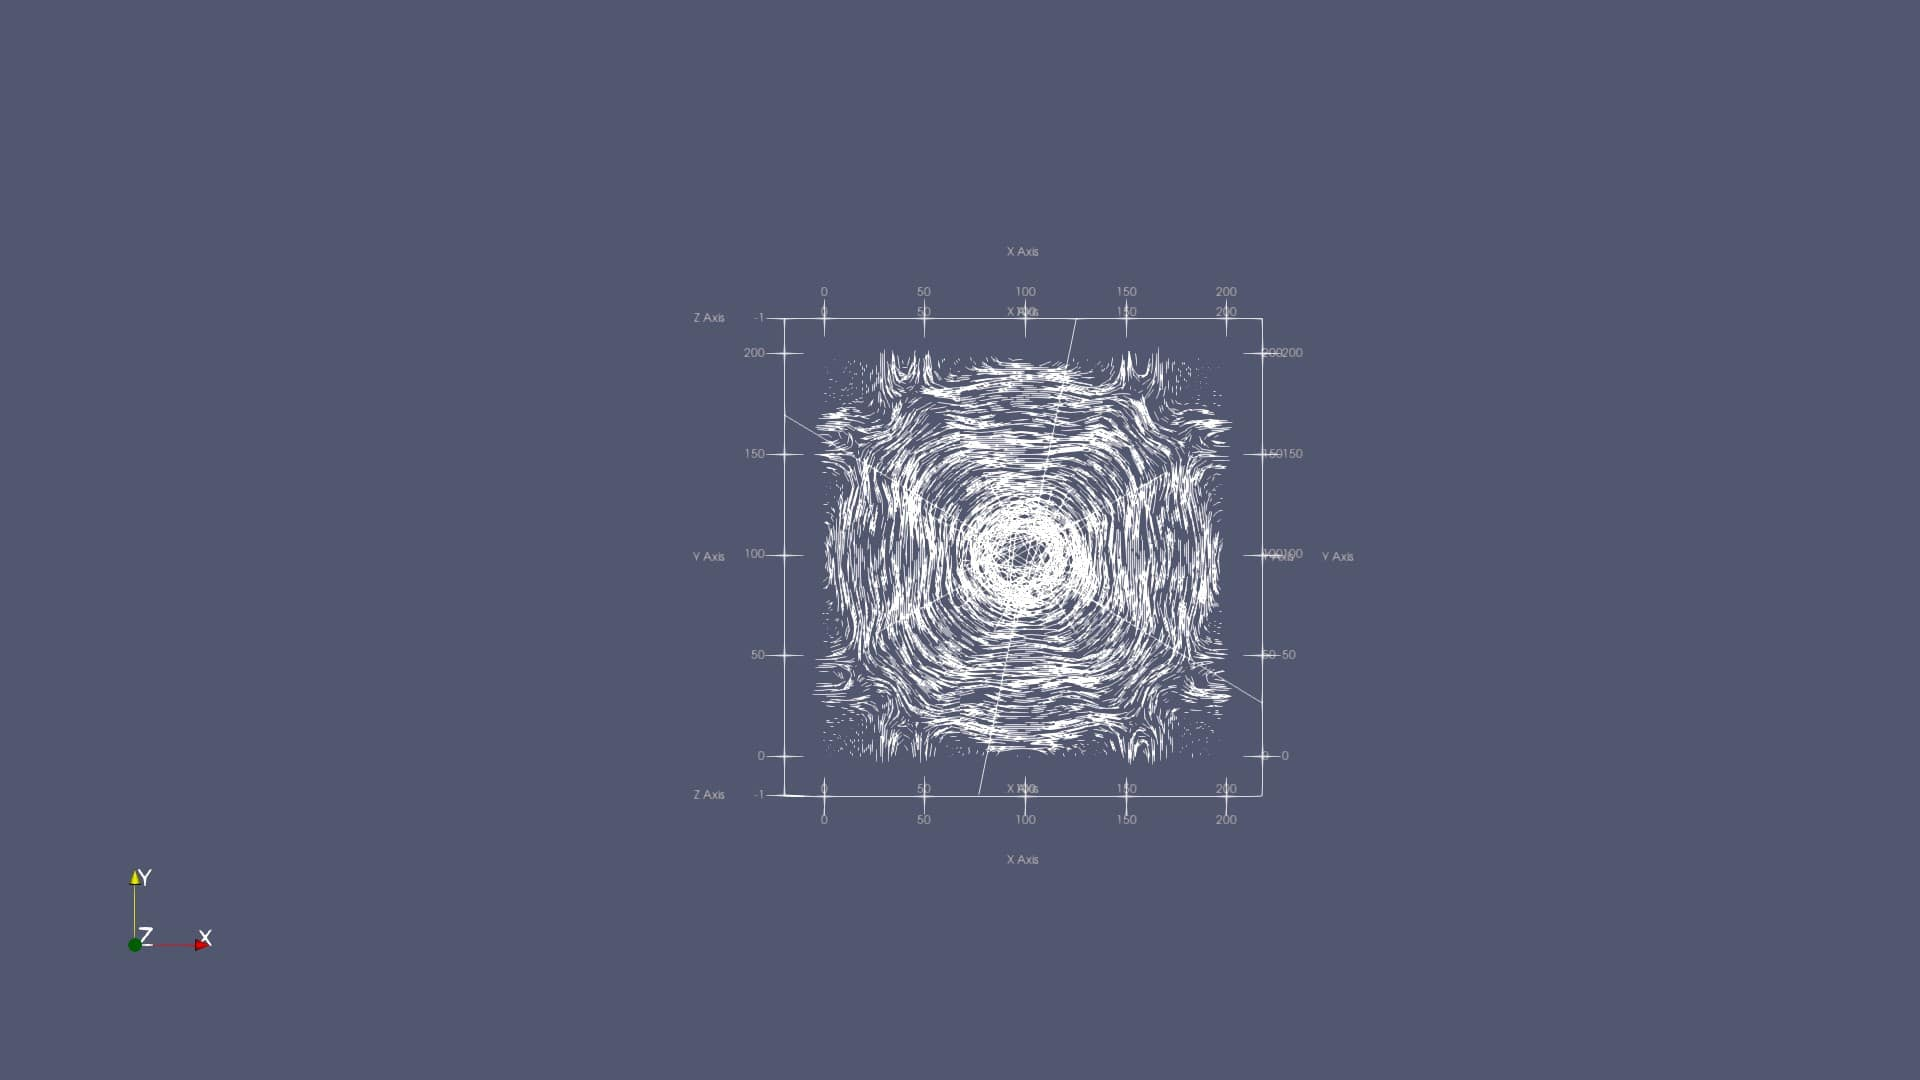
\includegraphics[width=.95\linewidth]{Figures/FDTD2DE4}
    	\caption{t = 800}
    \end{subfigure}
	\decoRule
	\caption[2D Electric Field Simulation]{A simulation of the 2D electric field.}
	\label{fig:FDTD2DE}
\end{figure}

The above is for the vectorial electric data. For the scalar magnetic data it may be more simple to use \textbf{Table to Structured Grid}. With a few adjustments to colors and scaling, the following result can be achieved (Figure \ref{fig:FDTD2DH}):

\begin{figure}[h!]
	\centering
	\begin{subfigure}{.49\textwidth}
		\centering
		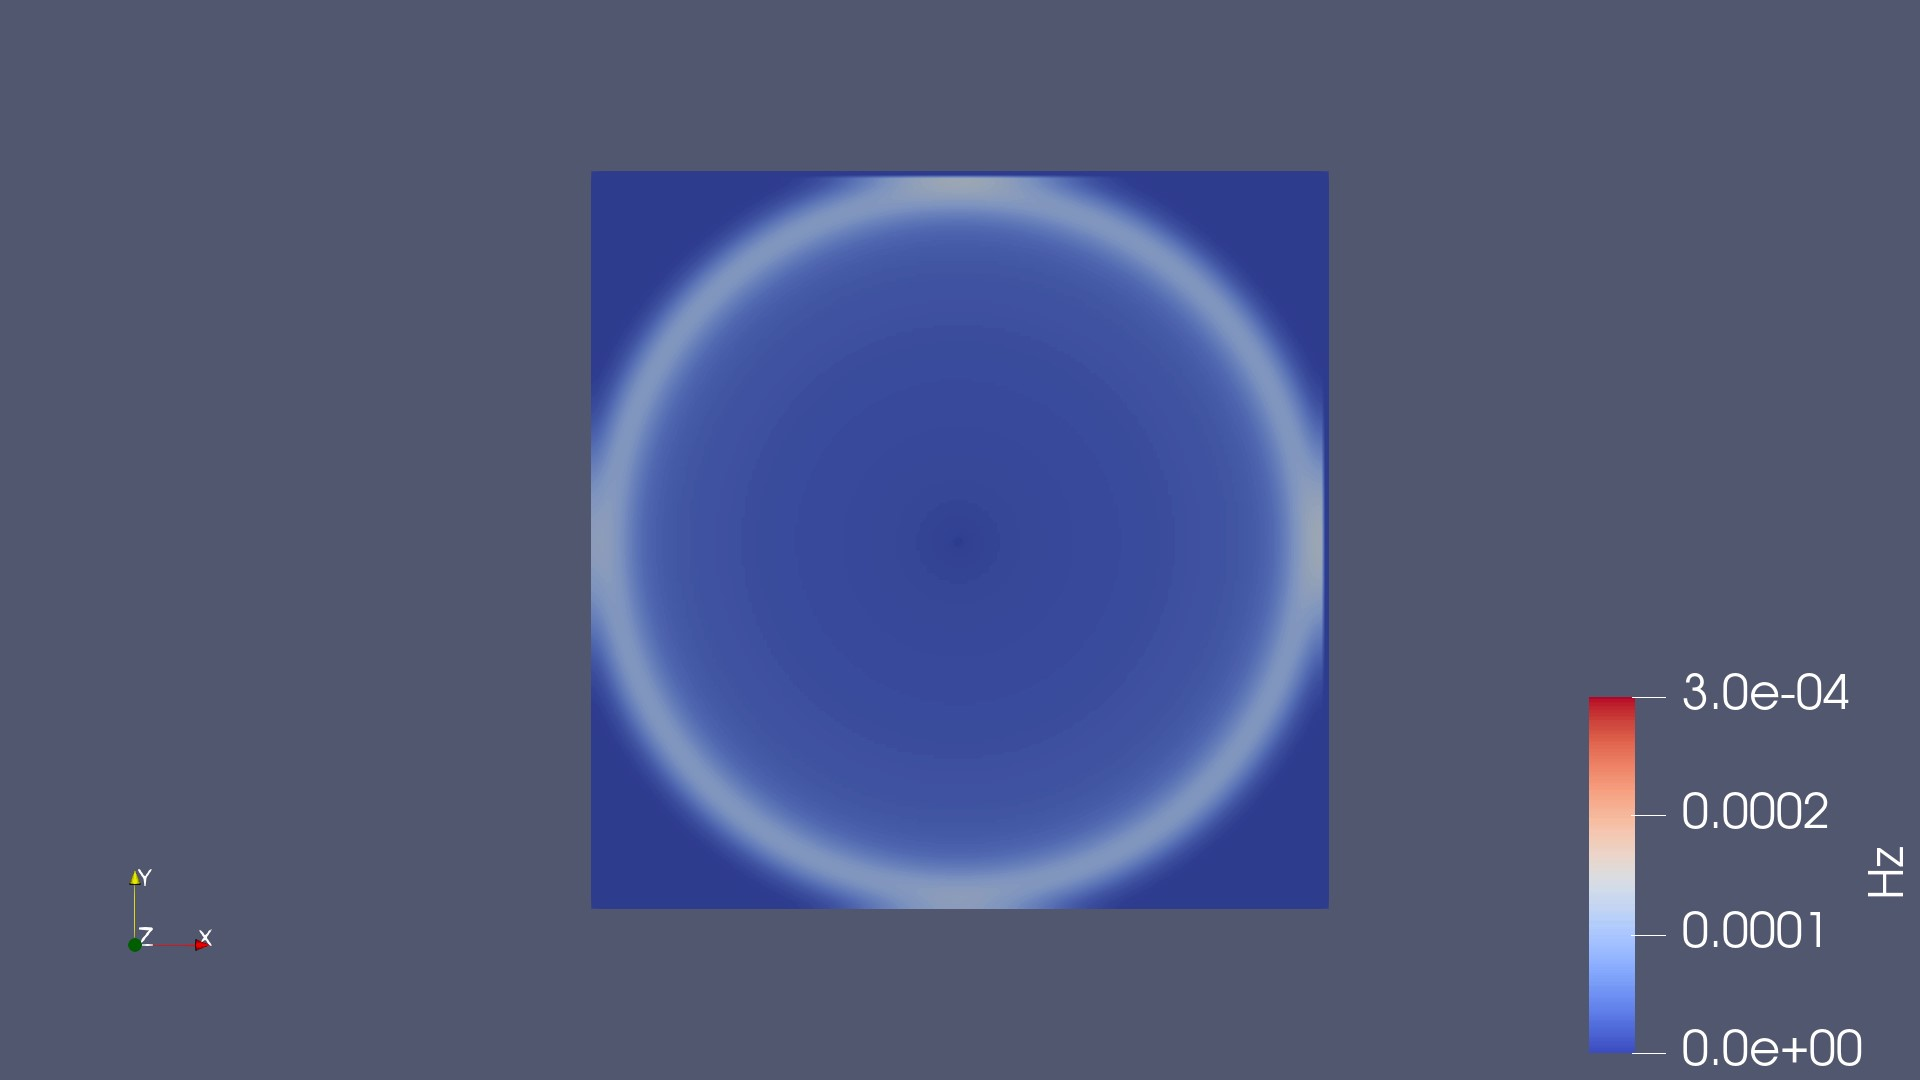
\includegraphics[width=.95\linewidth]{Figures/FDTD2DH1}
		\caption{t = 200}
	\end{subfigure}
	\begin{subfigure}{.49\textwidth}
		\centering
		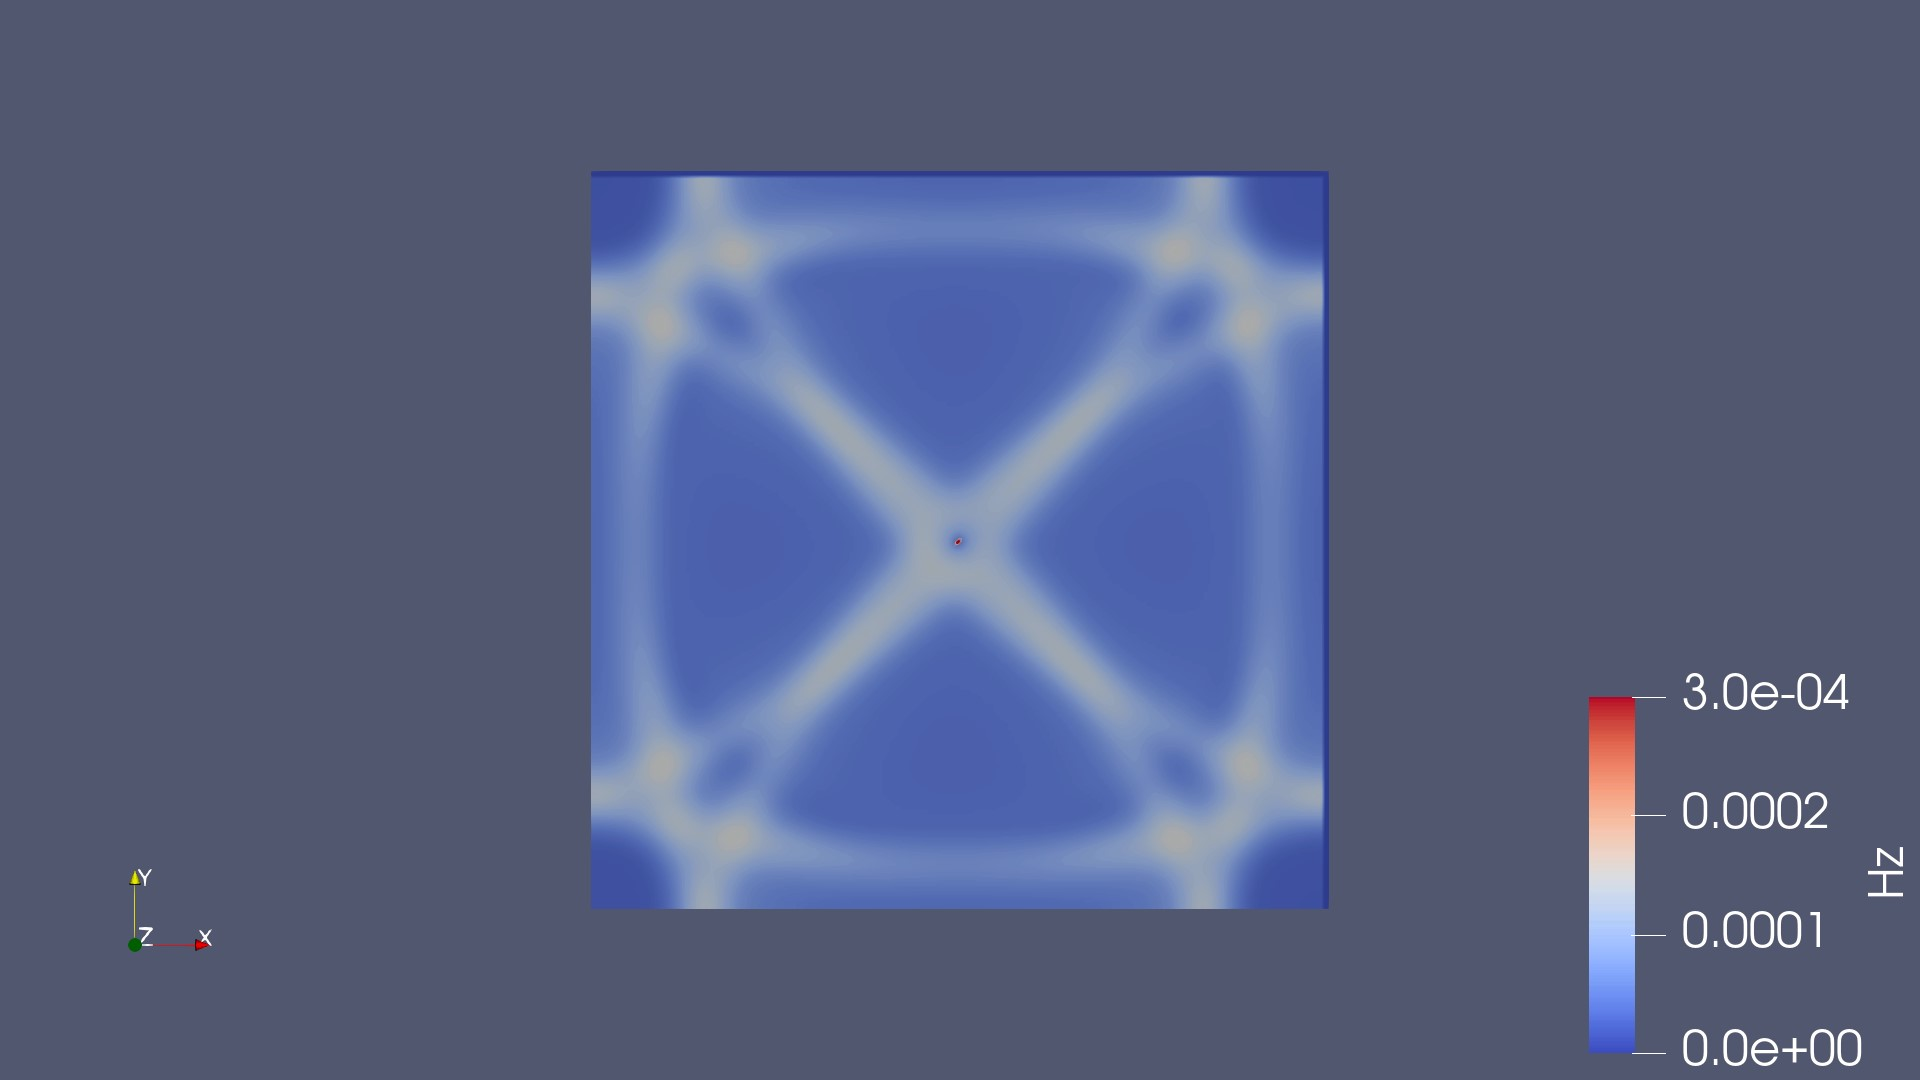
\includegraphics[width=.95\linewidth]{Figures/FDTD2DH2}
		\caption{t = 400}
	\end{subfigure}
	\begin{subfigure}{.49\textwidth}
		\centering
		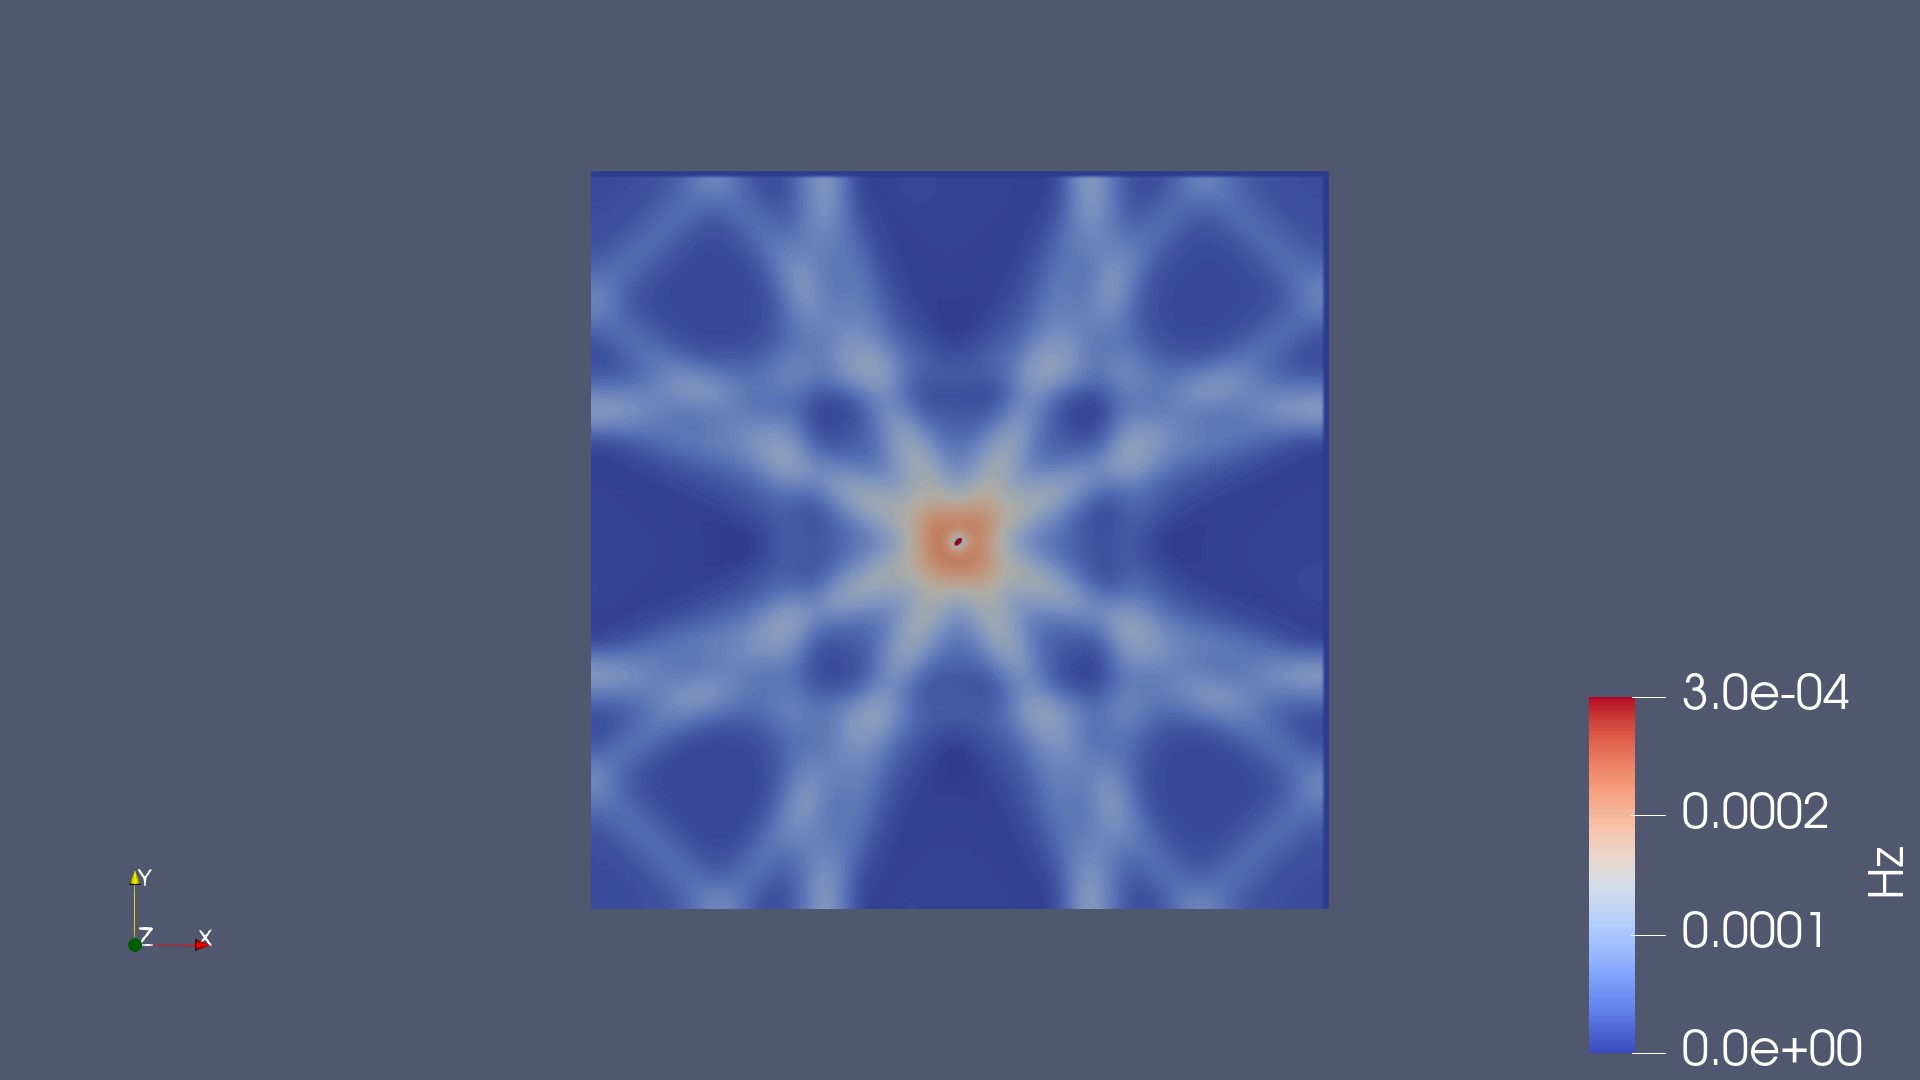
\includegraphics[width=.95\linewidth]{Figures/FDTD2DH3}
		\caption{t = 600}
	\end{subfigure}
	\begin{subfigure}{.49\textwidth}
		\centering
		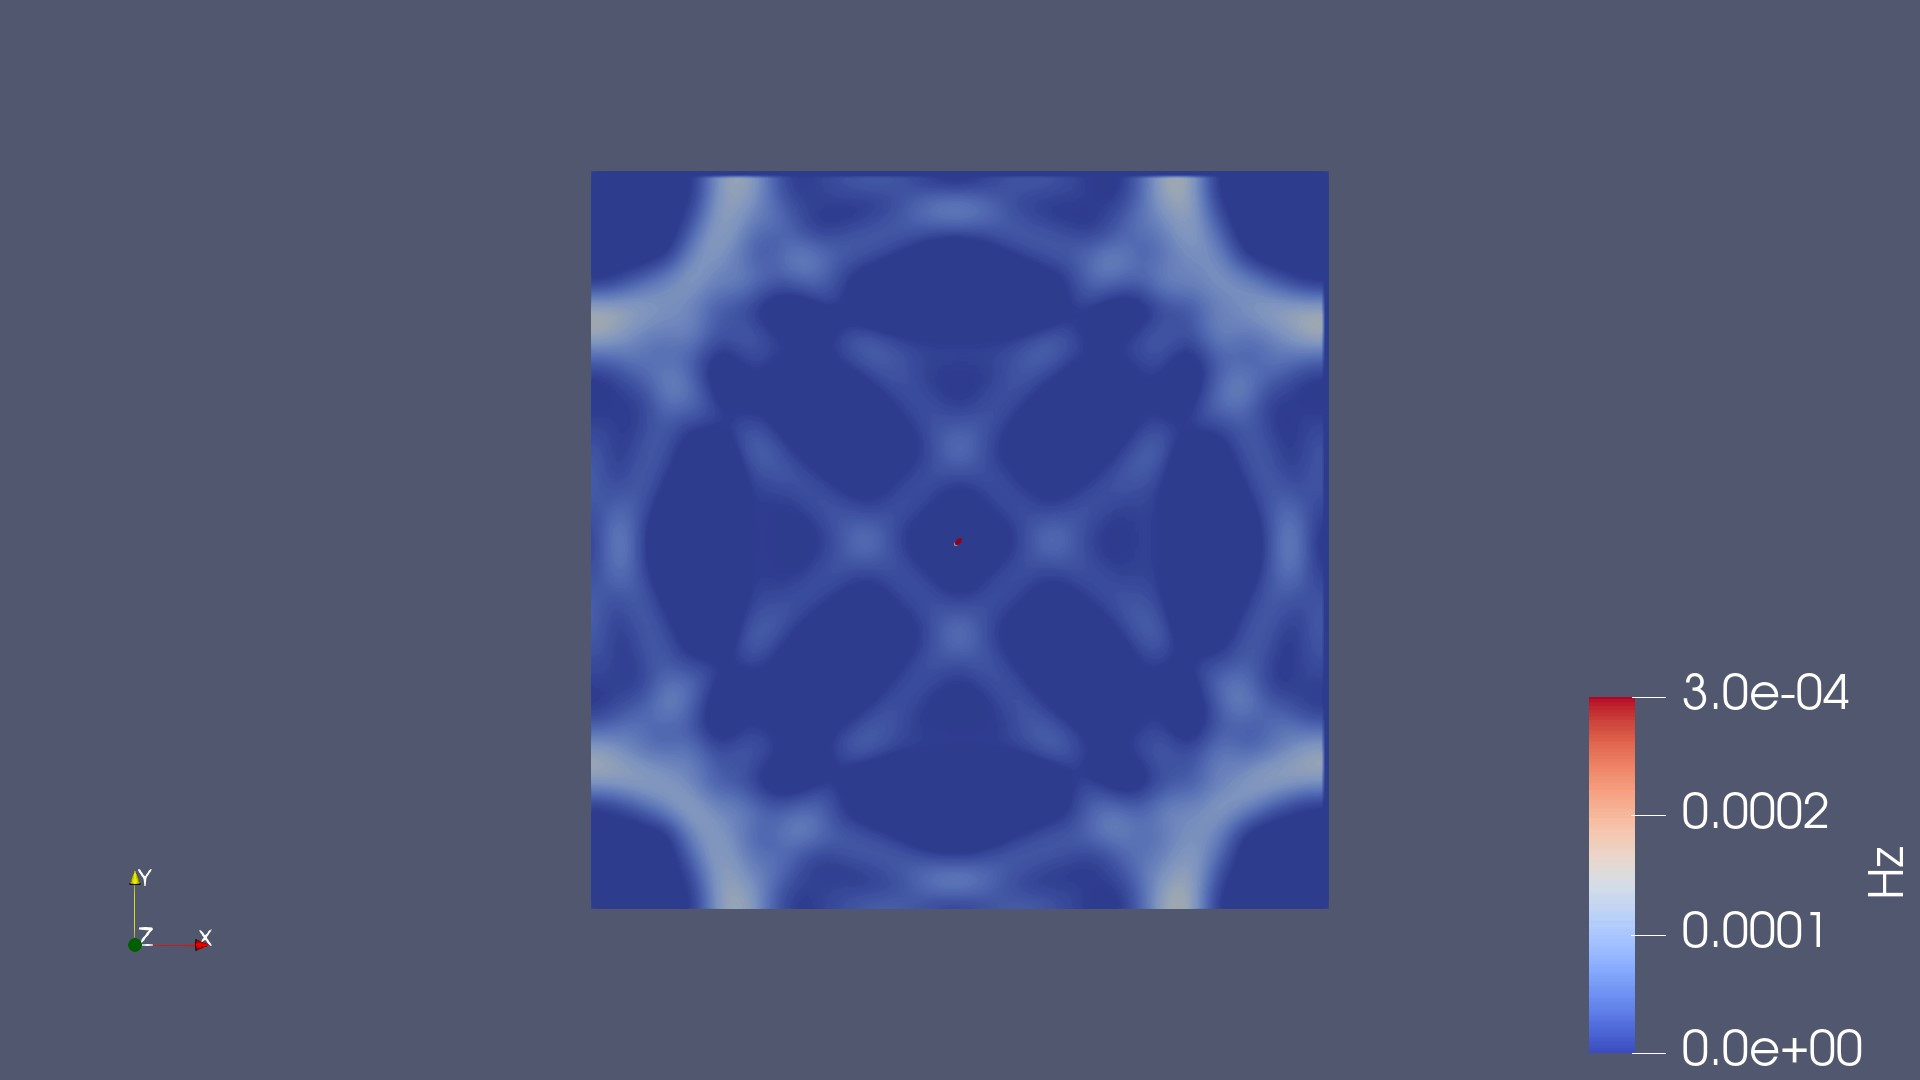
\includegraphics[width=.95\linewidth]{Figures/FDTD2DH4}
		\caption{t = 800}
	\end{subfigure}
	\decoRule
	\caption[2D Magnetic Field Simulation]{A simulation of the 2D magnetic field.}
	\label{fig:FDTD2DH}
\end{figure}

Moving forward, only the visualizing method for the electric data above can be of use, as the \textbf{Table to Structured Grid} method is not applicable when using more than one vector component. With that done, the three-dimensional scenario can finally be discussed, being the most useful one for practical real life applications.